\documentclass[conference]{IEEEtran}
\IEEEoverridecommandlockouts
% The preceding line is only needed to identify funding in the first footnote. If that is unneeded, please comment it out.
\usepackage{cite}
\usepackage{amsmath,amssymb,amsfonts}
\usepackage{algorithmic}
\usepackage{graphicx}
\usepackage{textcomp}
\usepackage{xcolor}
\def\BibTeX{{\rm B\kern-.05em{\sc i\kern-.025em b}\kern-.08em
    T\kern-.1667em\lower.7ex\hbox{E}\kern-.125emX}}
\begin{document}

\title{March Deliverables Report\\

\vspace{10pt}
\footnotesize{Establish best practices for data processing, system identification, and parameter estimation of the MHK energy device data using marine energy resource data, field test data, and simulation data to develop power flow dynamic models and their parameters in PSS®E.}

}

% \author{\IEEEauthorblockN{1\textsuperscript{st} Given Name Surname}
% \IEEEauthorblockA{\textit{dept. name of organization (of Aff.)} \\
% \textit{name of organization (of Aff.)}\\
% City, Country \\
% email address or ORCID}
% \and
% \IEEEauthorblockN{2\textsuperscript{nd} Given Name Surname}
% \IEEEauthorblockA{\textit{dept. name of organization (of Aff.)} \\
% \textit{name of organization (of Aff.)}\\
% City, Country \\
% email address or ORCID}
% \and
% \IEEEauthorblockN{3\textsuperscript{rd} Given Name Surname}
% \IEEEauthorblockA{\textit{dept. name of organization (of Aff.)} \\
% \textit{name of organization (of Aff.)}\\
% City, Country \\
% email address or ORCID}
% \and
% \IEEEauthorblockN{4\textsuperscript{th} Given Name Surname}
% \IEEEauthorblockA{\textit{dept. name of organization (of Aff.)} \\
% \textit{name of organization (of Aff.)}\\
% City, Country \\
% email address or ORCID}
% \and
% \IEEEauthorblockN{5\textsuperscript{th} Given Name Surname}
% \IEEEauthorblockA{\textit{dept. name of organization (of Aff.)} \\
% \textit{name of organization (of Aff.)}\\
% City, Country \\
% email address or ORCID}
% \and
% \IEEEauthorblockN{6\textsuperscript{th} Given Name Surname}
% \IEEEauthorblockA{\textit{dept. name of organization (of Aff.)} \\
% \textit{name of organization (of Aff.)}\\
% City, Country \\
% email address or ORCID}
% }

\maketitle

% \begin{abstract}
% \end{abstract}

% \begin{IEEEkeywords}

% \end{IEEEkeywords}

% \section{Thing to do}

% \begin{itemize}
%     \item How does other similar project and papers share and store data?
%     \item review Db paper, in this power systems context
%     \item kinda like a lit review, need to motivate our decisions
% % \end{itemize}

% \section{Introduction}
% don't think we need this for now


% \section{ignore - Milestone 5.2.2}

% \textbf{Establish best practices for data processing, system identification, and parameter estimation of the MHK energy device data using marine energy resource data, field test data, and simulation data to develop power flow dynamic models and their parameters in PSS®E.}

% This milestone aims to establish best practices for processing, identifying, and estimating parameters of marine hydrokinetic (MHK) energy device data to support dynamic power flow modeling in PSS®E and PowerDynamics.jl. The focus is on integrating marine energy resource data, field test data, and simulation data into a structured and accessible framework within the WEC-Grid software. This requires defining clear methodologies for data organization, retrieval, and processing to ensure consistency across simulations and analysis.

% \begin{figure}
%     \centering
%     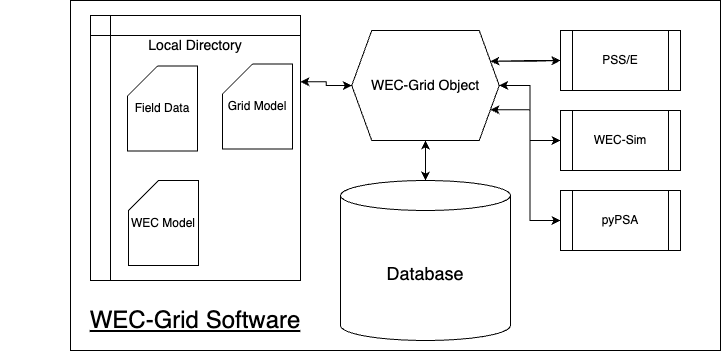
\includegraphics[width=\linewidth]{WEC_Grid_org.png} % Adjust path to your image
%     \caption{viz of org}
%     \label{fig:rm3_wec}
% \end{figure}


% \begin{figure}
%     \centering
%     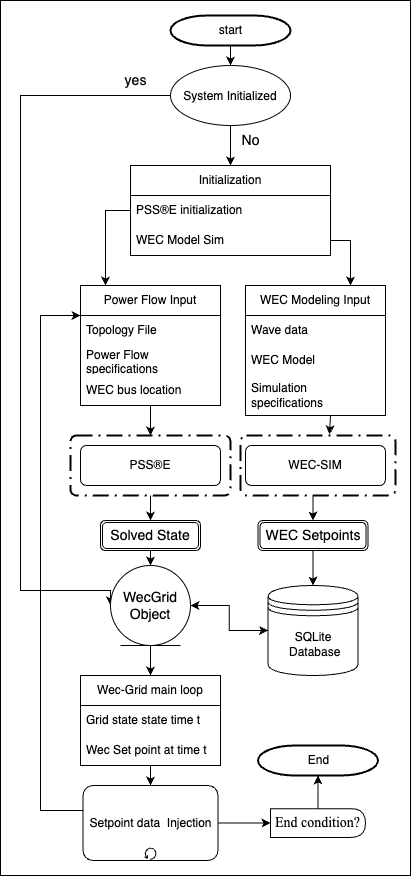
\includegraphics[width=0.8\linewidth]{data_flow.png} % Adjust path to your image
%     \caption{viz of org}
%     \label{fig:rm3_wec}
% \end{figure}

% To achieve this, all simulation and field test data should be centralized within an SQLite database, providing a unified structure for storing and querying results from WEC-SIM, WEC-Grid, and CEC simulations. While the raw grid topology and WEC-SIM MATLAB models remain in their native file formats, their associated metadata and outputs will be recorded in the database for accessibility. The database schema will include tables for identifying devices, simulations, and field test datasets, each with unique identifiers, descriptions, and relevant parameters. A dedicated table will catalog simulation metadata, allowing users to track details such as solver type, simulation resolution, and specific parameter settings. Example entries include identifiers for WEC-SIM simulations, field test datasets, and WEC-Grid power system studies, each linked to timestamps and parameter descriptions.

% Time series data for simulations and field tests will be stored separately within the database, with structured tables that include key output variables such as active and reactive power (P, Q), voltage magnitude (V), and additional state variables. WEC-SIM and field test datasets will follow a standardized format, where each time step corresponds to a specific power and voltage state. Similarly, WEC-Grid power system simulations will store snapshots of grid states, either as structured pandas dataframes or individual timestamped records. This ensures compatibility with both power flow solvers and marine energy models.
% The data processing workflow involves several key steps. First, data is ingested from multiple sources, including field test logs, marine energy resource datasets, and simulation outputs. Next, preprocessing ensures that all datasets conform to standardized formats, including required timestamp fields for synchronization. Processed results are then stored in the SQLite database for structured querying. The database will support version-controlled entries to track updates and allow users to compare multiple simulation runs. Figures 3 and 4 provide an overview of the data structure and the simulation processing pipeline, illustrating the flow from raw inputs to final dynamic power flow models.

% System identification within this framework refers to establishing consistent methods for recognizing and tracking different datasets. MHK devices, grid models, and simulations will be identified through unique filenames and IDs, ensuring that field test data, simulation results, and processed models can be easily referenced and retrieved. Each dataset will include metadata specifying device type, location (for field data), and relevant simulation parameters. Filenames and database identifiers will follow a structured naming convention, enabling automated tracking of simulation runs and their corresponding results.

% Parameter estimation is a key component of this milestone, particularly in defining the necessary coefficients for integrating MHK devices into power flow solvers. WEC-SIM output requires parameters such as hydrodynamic coefficients, drag values, and power take-off (PTO) characteristics, which are critical for modeling device behavior in grid simulations. Field test data contributes additional parameters, including device-specific damping characteristics and real-world performance metrics. For grid modeling, estimated parameters will include machine base power (MBase), active and reactive power outputs, and voltage and frequency response characteristics. These values will be systematically stored and linked to their respective simulations to facilitate integration into power system analysis tools.

% The best practices developed in this milestone will ensure a structured and reproducible methodology for handling MHK energy device data. By centralizing simulation and field test results within the WEC-Grid database, researchers and engineers can efficiently retrieve, process, and analyze datasets for dynamic power flow modeling. This approach supports ongoing research efforts in marine energy integration, providing a scalable and standardized foundation for future studies. Further refinement of database features, including user annotation capabilities and enhanced metadata tracking, will continue as part of the WEC-Grid development roadmap.





% \section{Deliverable 5.2.1}

% \textbf{Open-source PSS®E dynamic model of selected MHK device(s) with model agreement within 80\% target for similarity performance metrics.}

% Development of a model testbed has begun in PowerFactory. PowerFactory is a power flow simulation software comparable to PSS®E. The testbed will be used to verify MHK device model performance.
% To support this deliverable, the capabilities of the Julia-based PowerDynamics.jl package are being extended to process raw time-series field data. Unlike the existing WEC-Sim integration, which models device behavior using simulated data, this extension will allow the use of real field data, such as the raw UAF data generated for M5.2.1. Modifications to the PowerDynamics.jl source code are being further extended to enable compatibility with time-series inputs, ensuring it can simulate CEC device dynamics directly from the field data. Additionally, the approach will incorporate IEEE test cases alongside the UAF test case developed specifically for this project.
% This task builds on prior work done for the Dynamics paper, where a similar wrapper was developed to integrate WEC-Sim data into PowerDynamics.jl. The new model will bridge the gap between simulation and field data, allowing dynamic simulations to evaluate the performance and grid impact of MHK devices with real-world accuracy. By leveraging open-source tools, this effort provides a scalable and replicable framework for future MHK device studies.

\section{Deliverable 5.2.1}

\textbf{Open-source PSS®E dynamic model of selected MHK device(s) with model agreement within 80\% target for similarity performance metrics.}


\subsection{Introduction}
    \begin{itemize}
        \item Clarification of original deliverable goals (PSS®E dynamic model).
        \item Current implementation using PowerDynamics.jl (Julia-based) instead of PSS®E.
        \item Definition of ``model agreement'' for comparing the developed PowerDynamics.jl model to shuv's Simulink model.
    \end{itemize}

    To support this deliverable, the capabilities of the Julia-based PowerDynamics.jl package are being extended to process raw time series field data. 


\subsection*{Dynamic Models}

    \subsubsection*{Linear PTO WEC Model}
    
    The Linear Power Take-Off (PTO) model developed as part of deliverable 5.1.1 serves as the interface between the hydrodynamic motion of a Wave Energy Converter and its interaction with the power grid. 

    A brief overview of the dynamic PTO model development… The dynamic WEC integration is modeled in two stages: The Hydrodynamic Simulation (WEC-SIM) and then Grid Integration (PowerDynamics.jl). Using WEC-SIM, the WEC's motion is simulated using the Reference Model 3 (RM3), a two-body point absorber. WEC-SIM outputs key mechanical parameters, including Relative displacement ($X_{rel}$) between the float and spar, Relative velocity ($\dot{X}_{rel}$), representing the rate of change of displacement and Time-series wave elevation data.

    The PTO model is built ontop of PowerDynamics' VSIMinimal inverter model, allowing the simulation to use real-time relative displacement and velocity as inputs.

    The WEC-SIM outputs are post-processed and initialized with the dynamic PTO model, which is part of the larger dynamic power system model in PowerDynamics.jl. With our fork on PowerDynamics, the simulator integrates the WEC (or PTO) using the relative values to produce our generation. The simulation workflow, shown in Figure~\ref{fig:wec_pipeline}, illustrates the entire processing pipeline from wave simulation parameters to grid simulations. 
    
    \begin{figure}[h]
        \centering
        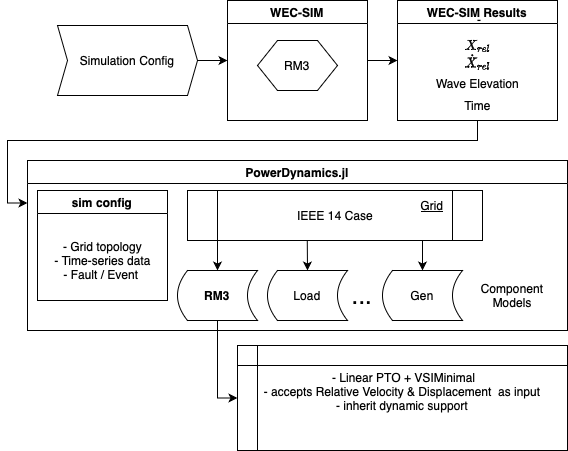
\includegraphics[width=0.9\linewidth]{Figs/pipeline.drawio-2.png}
        \caption{Simulation framework integrating WEC-SIM with PowerDynamics.jl for grid simulation.}
        \label{fig:wec_pipeline}
    \end{figure}
    
    A detailed breakdown of the PTO model equations, control strategy, and stability analysis is provided in Deliverable 5.1.1.

    
    \subsubsection*{Simulink WEC Dynamic Model}
        Description of the WEC Simulink model developed by Shuv.


   \subsubsection*{PowerDynamics.jl - IEEE14}

        The IEEE 14-bus system serves as the testbed for evaluating and comparing WEC integration into a power grid. We used a modified version of IEEE14 in deliverable 5.1.1 provided by PowerDynamics.jl with some additional modifications such as an additional WEC bus. 
        
        The default PowerDynamics.jl IEEE14 bus case is a PU ... need to describe how PowerDynamics implements their dynamic IEE14 model 
        
        We reused the default IEEE14 for this deliverable with some modifications to compare with the Simulink / power factor version ...  need to describe how we will potentially update the default model so we can compare in the next section
        
        
        With the discussed model parameter updates, this allows for a direct evaluation of how WEC integration impacts grid stability, frequency response, and power flow between both the Linear PTO and Simulink dynamics models.
        
    \subsubsection*{Simulink or PowerFactory - IEEE14}
        placeholder


\subsection*{Simulation}
    \subsubsection*{Set-up}
        \begin{itemize}
            \item Simulation length: 5 minutes.
            \item Time step resolution: 0.02 seconds.
            \item Load scenario: Constant load conditions.
            \item Wave conditions: 2.5-meter height, 8-second period.
            \item Additional agreed-upon initial conditions.
        \end{itemize}
        
    \subsubsection*{output}
        maybe here we can talk a little about our different outputs and how we plan to try to compare them. any assumptions too. 
    
\subsection*{Comparison Analysis (Performance Metrics of 80\%)}
    I'm a bit confused about what the 80\% means. 
    
    \subsubsection*{compare wec dynamics}

    \subsubsection*{compare grid dynamics}

    \subsubsection*{analysis}
        difference in how the grids responded.

% \subsection*{Discussion}
%     did we hit the Performance Metrics of 80\% ? 




\section{Deliverable 5.3.1}

\textbf{Report on a test system microgrid stability study with the developed power converter and system fault-protection model.}

We are currently developing a low-voltage ride-through (LVRT) mechanism for converters and a fault protection model for the Wave-to-Grid (W2G) system. The LVRT capability has been implemented in the grid-side converter (GSC) to handle symmetrical three-phase grid faults. The W2G model has been integrated into a simplified three-bus power system to evaluate its performance within a microgrid environment, as shown in Fig.[YC1]  8.
Additionally, efforts were made to connect and assess the stability of the developed W2G system with LVRT capability in the IEEE 13-bus standard test case. However, the desired performance was not achieved due to the unbalanced nature of the original IEEE 13-bus system. Work is currently underway to modify the test case and achieve a balanced configuration.
Ongoing efforts are focused on developing an effective control strategy for the W2G system to facilitate its integration into the target microgrid and conduct comprehensive stability tests.



\vspace{12pt}



% \section{Conclusion}
\end{document}
